\documentclass{../exhibit}

\title{Pirate Set}

%% Font
\usepackage{imfellEnglish}
\usepackage[T1]{fontenc}
\raggedright

\usepackage{background}

\backgroundsetup{
scale=1,
color=black,
opacity=0.4,
angle=0,
contents={%
  \includegraphics[height=\paperheight]{mapBackground.jpg}%%https://upload.wikimedia.org/wikipedia/commons/8/81/Nautical_chart_of_the_West_Indies_1797.jpg
  }%
}




%% For the context
%% https://tex.stackexchange.com/questions/86150/torn-page-effect/86151#86151
\usepackage{tikz}
\usetikzlibrary{decorations.pathmorphing}
\definecolor{paper}{RGB}{239,227,157}





\renewcommand{\maketitle}{ %
  \begin{center}
    \scalebox{8}{\thetitle}
  \end{center}
  
\begin{tabular*}{\textwidth}{c @{\extracolsep{\fill}} c}  
\resizebox{4in}{!}{\begin{minipage}[b]{3in}\huge\directions\end{minipage}} &
  \resizebox{4in}{!}{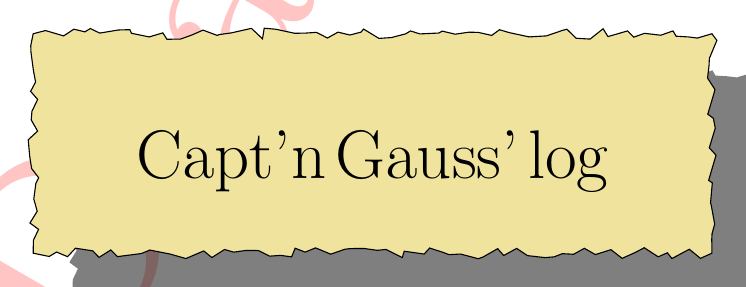
\begin{tikzpicture}[pencildraw/.style={ %
    decorate,
    decoration={random steps,segment length=4pt,amplitude=2pt}
    } %
]
\node[
preaction={fill=black,opacity=.5,transform canvas={xshift=.5cm,yshift=-.5cm}},
pencildraw,draw,fill=paper,text width=3in,inner sep=.5cm] 
{\begin{center}\Huge Capt'n Gauss' log \end{center}\vspace{.7cm} {\huge\context}};
\end{tikzpicture}}

\end{tabular*}

\vfill

\includegraphics[width=3in]{logoPirate.png}\hfill \includegraphics[width=2in]{bammLogo.png}


}


\begin{document}



\begin{context}
  Of all me $\pi$-rate games, I have one that is the best
  



  \vspace{1cm}

  SET


  \vspace{1cm}

  While it may seem simple, is pushes the imagination, like a sail pushes me boat!
\end{context}



\begin{directions}
  A SET is THREE CARDS with all satisfied:\huge
  \begin{itemize}
  \item They all have the same number OR \\have three different numbers.
  \item They all have the same shape OR \\have three different shapes.
  \item They all have the same shading OR\\ have three different shadings.
  \item They all have the same color OR\\ have three different colors.
  \end{itemize}
\end{directions}



\begin{example}%% image from https://medium.com/swlh/building-a-set-solver-using-python-and-opencv-4413389e7fdd
  \begin{center}
    \includegraphics[height=.3\textheight]{setgame.png}
    %% \begin{tabular}{lr}
    %%   \raisebox{-2in}{\includegraphics[width=.4\textwidth]{dots.png}} &
    %%   \quad\quad\begin{minipage}{.4\textwidth}
    %%     Here we see\\[1cm]
    %%     FIVE groups of TWO\\[1cm]
    %%     so there are TEN!
    %%   \end{minipage}
    %% \end{tabular}
  \end{center}
\end{example}




\begin{mathConnections}
  https://bartsnapp.github.io/Math-Outreach-Exhibits/count/
\end{mathConnections}
\end{document}
